%% ;;; -*- mode: Rnw; -*-
\documentclass{config/apuntes}\usepackage[]{graphicx}\usepackage[]{xcolor}
% maxwidth is the original width if it is less than linewidth
% otherwise use linewidth (to make sure the graphics do not exceed the margin)
\makeatletter
\def\maxwidth{ %
  \ifdim\Gin@nat@width>\linewidth
    \linewidth
  \else
    \Gin@nat@width
  \fi
}
\makeatother

\definecolor{fgcolor}{rgb}{0.345, 0.345, 0.345}
\newcommand{\hlnum}[1]{\textcolor[rgb]{0.686,0.059,0.569}{#1}}%
\newcommand{\hlsng}[1]{\textcolor[rgb]{0.192,0.494,0.8}{#1}}%
\newcommand{\hlcom}[1]{\textcolor[rgb]{0.678,0.584,0.686}{\textit{#1}}}%
\newcommand{\hlopt}[1]{\textcolor[rgb]{0,0,0}{#1}}%
\newcommand{\hldef}[1]{\textcolor[rgb]{0.345,0.345,0.345}{#1}}%
\newcommand{\hlkwa}[1]{\textcolor[rgb]{0.161,0.373,0.58}{\textbf{#1}}}%
\newcommand{\hlkwb}[1]{\textcolor[rgb]{0.69,0.353,0.396}{#1}}%
\newcommand{\hlkwc}[1]{\textcolor[rgb]{0.333,0.667,0.333}{#1}}%
\newcommand{\hlkwd}[1]{\textcolor[rgb]{0.737,0.353,0.396}{\textbf{#1}}}%
\let\hlipl\hlkwb

\usepackage{framed}
\makeatletter
\newenvironment{kframe}{%
 \def\at@end@of@kframe{}%
 \ifinner\ifhmode%
  \def\at@end@of@kframe{\end{minipage}}%
  \begin{minipage}{\columnwidth}%
 \fi\fi%
 \def\FrameCommand##1{\hskip\@totalleftmargin \hskip-\fboxsep
 \colorbox{shadecolor}{##1}\hskip-\fboxsep
     % There is no \\@totalrightmargin, so:
     \hskip-\linewidth \hskip-\@totalleftmargin \hskip\columnwidth}%
 \MakeFramed {\advance\hsize-\width
   \@totalleftmargin\z@ \linewidth\hsize
   \@setminipage}}%
 {\par\unskip\endMakeFramed%
 \at@end@of@kframe}
\makeatother

\definecolor{shadecolor}{rgb}{.97, .97, .97}
\definecolor{messagecolor}{rgb}{0, 0, 0}
\definecolor{warningcolor}{rgb}{1, 0, 1}
\definecolor{errorcolor}{rgb}{1, 0, 0}
\newenvironment{knitrout}{}{} % an empty environment to be redefined in TeX

\usepackage{alltt}

\title{Programación y Estadística con R}
\author{Sandra Mingo Ramírez}
\date{2024/25}
\acronym{PRSTR}

\usepackage[all]{nowidow}
\usepackage{listing}
\usepackage{color}
\usepackage{tabularx}
\usepackage{multirow}
\usepackage{makecell}
\usepackage{amsmath}
\usepackage{array}



\IfFileExists{upquote.sty}{\usepackage{upquote}}{}
\begin{document}

\begin{abstract}
Este curso es una introducción rápida a un «entorno para la computación estadística y los gráficos», que proporciona una amplia variedad de técnicas estadísticas y gráficas: modelización lineal y no lineal, pruebas estadísticas, análisis de series temporales, clasificación, agrupación, etc. Prácticamente todos los análisis estadísticos que se realizan en Bioinformática se pueden llevar a cabo con R. Además, la «minería de datos» está bien cubierta en R: el clustering (a menudo llamado «análisis no supervisado») en muchas de sus variantes (jerárquico, k-means y familia, modelos de mezcla, fuzzy, etc), bi-clustering, clasificación y discriminación (desde el análisis discriminante a los árboles de clasificación, bagging, máquinas de vectores soporte, etc), todos tienen muchos paquetes en R. Así, tareas como la búsqueda de subgrupos homogéneos en conjuntos de genes/sujetos, la identificación de genes que muestran una expresión diferencial (con ajuste para pruebas múltiples), la construcción de algoritmos de predicción de clases para separar a los pacientes de buen y mal pronóstico en función del perfil genético, o la identificación de regiones del genoma con pérdidas/ganancias de ADN (alteraciones del número de copias) pueden llevarse a cabo en R de forma inmediata.
\end{abstract}

\pagestyle{plain}

\maketitle

\tableofcontents


%Quick intro to R and a minimal of stats
%R programming with a modicum of stats
%Statistics with R: linear models
%Intro to causal inference
%Stats for omics

%Ejercicio de programación (40%) y dos exámenes parciales (30% cada uno)
%Ejercicio de programación en grupos de 3 o 4 personas, presentación de 13 minutos por grupo
%Evitar tidyverse

%09/10 - Ramón Díaz
\chapter{Introducción en R y estadística}
\section{RStudio y primeras nociones}
En RStudio, se puede crear un nuevo fichero en File > New File > R script. Se abre un nuevo fichero en el que se puede programar. En R, la asignación de variables se realiza con <-. En la parte superior derecha, se pueden ver todas las variables que se han asignado en la sesión, los datos y las funciones.

\begin{knitrout}
\definecolor{shadecolor}{rgb}{0.969, 0.969, 0.969}\color{fgcolor}\begin{kframe}
\begin{alltt}
\hldef{x} \hlkwb{<-} \hlnum{9}
\hldef{y} \hlkwb{<-} \hlkwd{matrix}\hldef{(}\hlnum{1}\hlopt{:}\hlnum{20}\hldef{,} \hlkwc{ncol} \hldef{=} \hlnum{4}\hldef{)}
\end{alltt}
\end{kframe}
\end{knitrout}

En la parte inferior derecha hay una pestaña para poder visualizar los gráficos. Desde ese menú, se puede guardar, pero esto no es recomendable, ya que el gráfico se ajusta al tamaño de la pantalla y luego eso no es reproducible. En otra pestaña aparece un listado de todos los paquetes instalados en el disco duro, aunque luego haya que cargarlos en cada script en el que se desee usar. Al pulsar en el nombre de un paquete, se va a la página de ayuda del mismo. También es posible acceder con:

\begin{knitrout}
\definecolor{shadecolor}{rgb}{0.969, 0.969, 0.969}\color{fgcolor}\begin{kframe}
\begin{alltt}
\hlkwd{help}\hldef{(rnorm)}
\end{alltt}
\end{kframe}
\end{knitrout}

La mayor parte del trabajo «real» con R requerirá la instalación de paquetes. Los paquetes proporcionan funcionalidad adicional. Los paquetes están disponibles en muchas fuentes diferentes, pero posiblemente las principales ahora son CRAN y BioConductor. Si un paquete está disponible en CRAN, puedes hacer lo siguiente:

\begin{knitrout}
\definecolor{shadecolor}{rgb}{0.969, 0.969, 0.969}\color{fgcolor}\begin{kframe}
\begin{alltt}
\hlkwd{install.packages}\hldef{(}\hlsng{"nombre-paquete"}\hldef{)} \hlcom{# 1 paquete}
\hlkwd{install.packages}\hldef{(}\hlkwd{c}\hldef{(}\hlsng{"paquete1"}\hldef{,} \hlsng{"paquete2"}\hldef{))} \hlcom{# varios paquetes}
\end{alltt}
\end{kframe}
\end{knitrout}

En Bioinformática, BioConductor es una fuente bien conocida de muchos paquetes diferentes. Los paquetes de BioConductor pueden instalarse de varias maneras, y existe una herramienta semiautomatizada que permite instalar conjuntos de paquetes BioC. Implican hacer algo como

\begin{knitrout}
\definecolor{shadecolor}{rgb}{0.969, 0.969, 0.969}\color{fgcolor}\begin{kframe}
\begin{alltt}
\hldef{BiocManager}\hlopt{::}\hlkwd{install}\hldef{(}\hlsng{"nombre-paquete"}\hldef{)}
\end{alltt}
\end{kframe}
\end{knitrout}

A veces los paquetes dependen de otros paquetes. Si este es el caso, por defecto, los mecanismos anteriores también instalarán las dependencias. Con algunas interfaces gráficas de usuario (en algunos sistemas operativos) también puede instalar paquetes desde una entrada de menú. Por ejemplo, en Windows, hay una entrada en la barra de menú llamada Paquetes, que permite instalar desde Internet, cambiar los repositorios, instalar desde archivos zip locales, etc. Del mismo modo, desde RStudio hay una entrada para instalar paquetes (en «Herramientas»). Los paquetes también están disponibles desde otros lugares (RForge, github, etc); a menudo encontrarás instrucciones allí.

Siempre puedes simplemente matar RStudio; pero eso no es agradable. En todos los sistemas escribir q() en el símbolo del sistema debería detener R/RStudio. También habrá entradas de menú (por ejemplo, «Salir de RStudio» en «Archivo», etc). A continuación sale la pregunta de si se debe guardar el workspace, y en general querremos decir que no.

\section{Ejemplo}
\subsection{Introducción al test de la t}
En un test de la t, la hipótesis nula ($H_0$) suele representar lo contrario de lo que se desea demostrar. Por ejemplo, si nuestro objetivo es comprobar si hay diferencias entre dos muestras, la hipótesis nula establece que ambas son iguales. A continuación, se utiliza la fórmula de la t para obtener un valor estadístico, cuya distribución se examina bajo la suposición de que $H_0$ es cierta. Luego, se calcula la probabilidad de observar un resultado tan extremo o más extremo que el obtenido bajo $H_0$. Esta probabilidad se denomina p-valor, y su interpretación indica cuánta evidencia hay en contra de $H_0$: un p-valor bajo sugiere que lo observado es improbable bajo $H_0$.

\[
t = \frac{x_A - x_B}{SD_{x_A, x_B}}
\]

Es importante aclarar que el p-valor no representa la probabilidad de que $H_0$ sea cierta, ni la probabilidad de que $H_0$ o la hipótesis alternativa ($H_1$) se cumplan dado los datos. Lo que el p-valor señala es que, o bien $H_0$ es falsa, o ha ocurrido un evento tan improbable como el valor observado. No se "rechaza" $H_0$ de manera concluyente, sino que simplemente no se acepta si el p-valor es suficientemente bajo. En este análisis, se compara el resultado observado con todos aquellos más extremos, algo que es distinto de seleccionar el valor que hace los datos lo más probables posible (como se hace en la máxima verosimilitud).

Por ejemplo, una moneda perfectamente equilibrada tiene una probabilidad de $0.5^6$ de que al lanzarla seis veces, salga exactamente tres veces cara y tres veces cruz. Aunque este número es pequeño, no implica que la hipótesis alternativa sea necesariamente más probable, ya que otros resultados también podrían ser igualmente o más improbables. En la mayoría de los casos de comparación de medias, los datos no están restringidos a un único valor.

Cuando $H_0$ es cierta:
$$Pr(p-valor \leq 0,05) = 0,05$$
$$Pr(p-valor \leq 0,01) = 0,01$$

En muchos casos se comprueba más de una $H_0$. En un screening, se analizan 20.000 genes y se decide elegir todos aquellos que tengan un p-valor inferior a 0,05. Esa lista, sobre el total de los genes, la probabilidad de rechazar $H_0$ cuando es cierta, es muy superior al 5\%, aunque se cumpla para cada gen individual. Así, se debe trasladar la lógica al test múltiple, puesto que si no se va a rechazar $H_0$ en muchas ocasiones cuando no se debería.

\subsection{Problema de las pruebas múltiples}
Es posible que hayamos oído hablar del problema de las pruebas múltiples con los microarrays: si observamos los p-valores de un gran número de pruebas, podemos ser inducidos a pensar erróneamente que está ocurriendo algo (es decir, que hay genes expresados de forma diferencial) cuando, en realidad, no hay absolutamente ninguna señal en los datos. A nosotros esto nos convence. Pero tienes un colega testarudo que no lo está. Ha decidido utilizar un ejemplo numérico sencillo para mostrarle el problema. Este es el escenario ficticio: 50 sujetos, de los cuales 30 tienen cáncer y 20 no. Medimos 1000 genes, pero ninguno de los genes tiene diferencias reales entre los dos grupos; para simplificar, todos los genes tienen la misma distribución (una distribución normal). Haremos una prueba t por gen, mostrará un histograma de los valores p e informaremos del número de genes «significativos» (genes con p < 0,05). Este es el código R:

\begin{knitrout}
\definecolor{shadecolor}{rgb}{0.969, 0.969, 0.969}\color{fgcolor}\begin{kframe}
\begin{alltt}
\hldef{randomdata} \hlkwb{<-} \hlkwd{matrix}\hldef{(}\hlkwd{rnorm}\hldef{(}\hlnum{50} \hlopt{*} \hlnum{1000}\hldef{),} \hlkwc{ncol} \hldef{=} \hlnum{50}\hldef{)}
\hldef{class} \hlkwb{<-} \hlkwd{factor}\hldef{(}\hlkwd{c}\hldef{(}\hlkwd{rep}\hldef{(}\hlsng{"NC"}\hldef{,} \hlnum{20}\hldef{),} \hlkwd{rep}\hldef{(}\hlsng{"cancer"}\hldef{,} \hlnum{30}\hldef{)))}
\hldef{pvalues} \hlkwb{<-} \hlkwd{apply}\hldef{(randomdata,} \hlnum{1}\hldef{,}
                 \hlkwa{function}\hldef{(}\hlkwc{x}\hldef{)} \hlkwd{t.test}\hldef{(x} \hlopt{~} \hldef{class)}\hlopt{$}\hldef{p.value)}
\end{alltt}
\end{kframe}
\end{knitrout}

Para leer el código, se empieza por la función más interna, que en este caso es \texttt{rnorm}. Así, primero se generan 50.000 entradas de distribución normal (1000 genes por 50 personas) de los que se quiere realizar 1000 contrastes de hipótesis (uno por gen) y representar el aspecto de la distribución (que será uniforme). Todas las entradas se organizan en una matriz con 50 columnas. Después, se crean los dos grupos que se están analizando mediante repeticiones (función \texttt{rep}). El comando de \texttt{factor} crea las etiquetas. En R, se puede llamar al test de la t de varias maneras, siendo una estándar con la interfaz de tipo fórmula (x $\sim$ class), dividiendo así x en los distintos niveles que se han creado previamente. La sintaxis siempre es una variable que va cambiando (en este caso, las filas) antes de la virgulilla y una variable constante después de la virgulilla (los distintos niveles). La función \texttt{apply} permite aplicar una función a un objeto o conjunto de datos, evitando así tener que realizar un bucle for. El primer argumento es el objeto, el segundo la dimensión del objeto a lo que se quiere aplicar (si se recorren filas, columnas, etc.), y el tercero la función que se va a aplicar. La función \texttt{t.test} devuelve objetos a los que se puede acceder, como el valor t, df, p-valor, la media de cada grupo, etc. Se puede acceder al nombre de todos los valores mediante \texttt{names(t.test(x $\sim$ class))}. En nuestro caso, x es el valor que irá adquiriendo el número de filas a recorrer. En este caso, se define la función en el momento de llamarla, pero también se puede definir antes y utilizarla en el apply. En este caso se define dentro porque es una función corta que solo se utilizará en ese momento, por lo que no es necesario crearla fuera. Si por el contrario fuese una función a la que quisiéramos acceder posteriormente o que fuese compleja con varias líneas, se suele crear fuera. Por último, se accede a los p-valores y se guardan en la variable \texttt{pvalues}. Esos p-valores se pueden representar a continuación en un histograma y calcular todos aquellos que sean menores o iguales que 0,05.

\begin{knitrout}
\definecolor{shadecolor}{rgb}{0.969, 0.969, 0.969}\color{fgcolor}\begin{kframe}
\begin{alltt}
\hlkwd{hist}\hldef{(pvalues)}
\end{alltt}
\end{kframe}
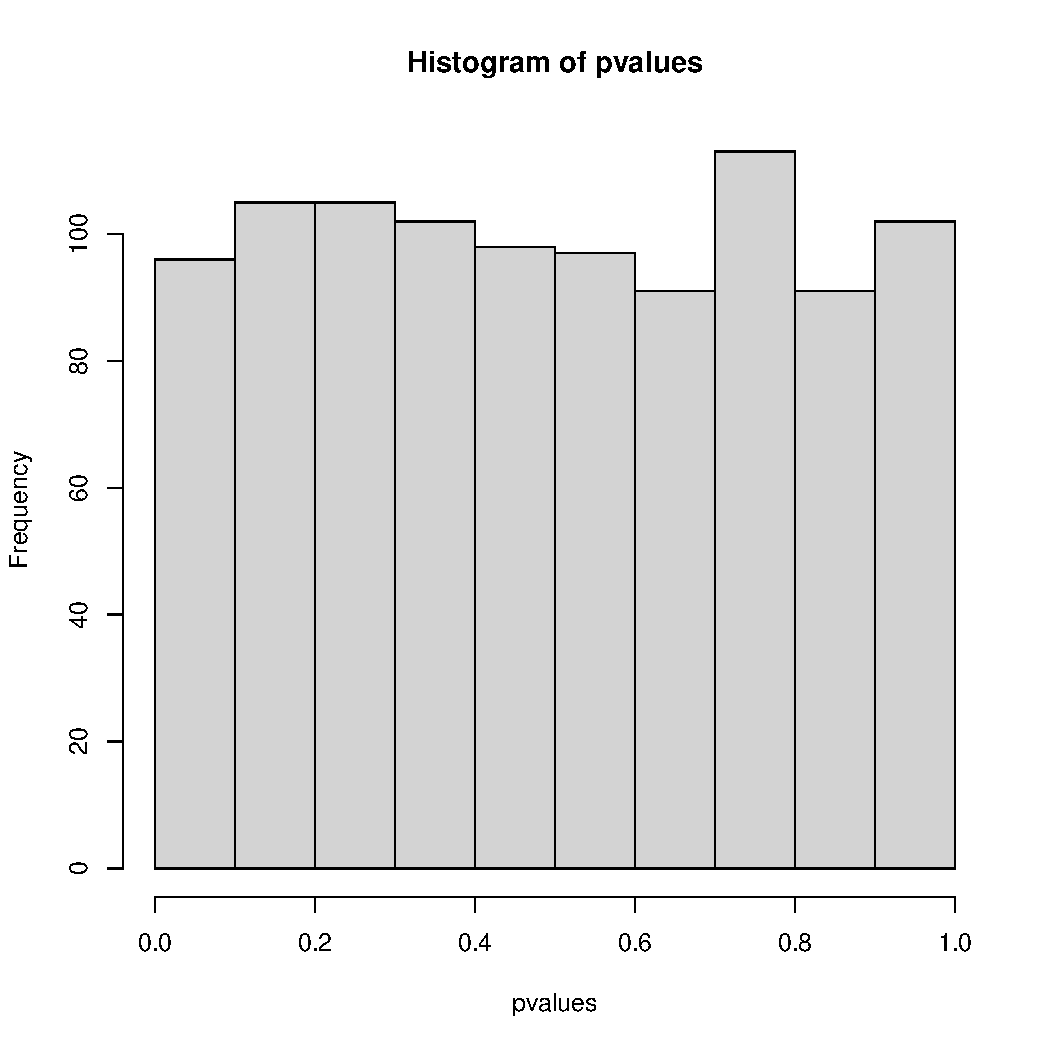
\includegraphics[width=\maxwidth]{figure/unnamed-chunk-7-1} 
\begin{kframe}\begin{alltt}
\hlkwd{sum}\hldef{(pvalues} \hlopt{<=} \hlnum{0.05}\hldef{)}
\end{alltt}
\begin{verbatim}
## [1] 43
\end{verbatim}
\end{kframe}
\end{knitrout}

Al realizar la suma de una lógica booleana, se coercia para que los valores falsos se conviertan en 0 y los verdaderos en 1. Así, al sumarlos, el resultado es numérico. 

En resumen, en este ejemplo hemos visto los siguientes objetos:
\begin{itemize}
\item Vectores: colección de uno o más datos del mismo tipo.
\item Matrices: conjunto de datos indexados por filas y columnas del mismo tipo. 
\item Arrays: generalización de una matriz que no tiene límite de dimensiones (pero debe tener una estrucrtura rectangular). 
\item Data frames: estructura rectangular de dos dimensiones (filas y columnas) en la que cada columna puede ser de un tipo diferente. 
\item Listas: cajón desastre en el que se pueden meter muchas cosas de muchos tipos distintos. Muchas funciones devuelven listas u objetos que contienen listas.
\item Factores: vectores de un tipo especial (variable categórica).
\item Funciones: objetos que realizan una operación y devuelven algo. 
\end{itemize}

En el siguiente código se muestran las distintas maneras de acceder a una matriz. La indexación funciona [filas, columnas], y si un campo está sin rellenar implica todos sus datos.

\begin{knitrout}
\definecolor{shadecolor}{rgb}{0.969, 0.969, 0.969}\color{fgcolor}\begin{kframe}
\begin{alltt}
\hldef{randomdata[}\hlnum{1}\hldef{, ]}
\hldef{randomdata[,} \hlnum{1}\hldef{]}
\hldef{randomdata[}\hlnum{2}\hldef{, ]}
\hldef{randomdata[,} \hlnum{2}\hldef{]}
\hldef{randomdata[}\hlnum{2}\hldef{,} \hlnum{3}\hldef{]}
\end{alltt}
\end{kframe}
\end{knitrout}

Al ejecutar la variable \texttt{class} creada anteriormente, no solo devuelve la lista de los elementos con las distintas etiquetas, si no que también muestra al final los distintos niveles. Como \texttt{factor} por detrás les asignó un valor entero que corresponda a la etiqueta dada, cuando se pide convertir en numérico, se devuelve el entero. La asignación de los valores se realiza por orden alfanumérico.

\begin{knitrout}
\definecolor{shadecolor}{rgb}{0.969, 0.969, 0.969}\color{fgcolor}\begin{kframe}
\begin{alltt}
\hldef{class}
\hlkwd{as.numeric}\hldef{(class)}
\end{alltt}
\end{kframe}
\end{knitrout}



\begin{knitrout}
\definecolor{shadecolor}{rgb}{0.969, 0.969, 0.969}\color{fgcolor}\begin{kframe}
\begin{alltt}
\hldef{pvalues[}\hlnum{1}\hldef{]}

\hlkwd{t.test}\hldef{(randomdata[}\hlnum{1}\hldef{, ]} \hlopt{~} \hldef{class)}

\hlkwd{t.test}\hldef{(randomdata[}\hlnum{1}\hldef{, ]} \hlopt{~} \hldef{class)}\hlopt{$}\hldef{p.value}

\hldef{pvalues[}\hlnum{1}\hlopt{:}\hlnum{10}\hldef{]} \hlopt{<} \hlnum{0.05}

\hlkwd{sum}\hldef{(}\hlkwd{c}\hldef{(}\hlnum{TRUE}\hldef{,} \hlnum{TRUE}\hldef{,} \hlnum{FALSE}\hldef{))}

\hlkwd{hist}\hldef{(}\hlkwd{c}\hldef{(}\hlnum{1}\hldef{,} \hlnum{2}\hldef{,} \hlnum{7}\hldef{,} \hlnum{7}\hldef{,} \hlnum{7}\hldef{,} \hlnum{8}\hldef{,} \hlnum{8}\hldef{))}
\end{alltt}
\end{kframe}
\end{knitrout}

\begin{knitrout}
\definecolor{shadecolor}{rgb}{0.969, 0.969, 0.969}\color{fgcolor}\begin{kframe}
\begin{alltt}
\hlcom{## For ease}
\hldef{rd2} \hlkwb{<-} \hldef{randomdata[}\hlnum{1}\hlopt{:}\hlnum{10}\hldef{, ]}

\hlcom{## Where we will store results}
\hldef{pv2} \hlkwb{<-} \hlkwd{vector}\hldef{(}\hlkwc{length} \hldef{=} \hlnum{10}\hldef{)}

\hlkwa{for}\hldef{(i} \hlkwa{in} \hlnum{1}\hlopt{:}\hlnum{10}\hldef{) \{}
    \hldef{pv2[i]} \hlkwb{<-} \hlkwd{t.test}\hldef{(rd2[i, ]} \hlopt{~} \hldef{class)}\hlopt{$}\hldef{p.value}
\hldef{\}}

\hldef{pv2}

\hlcom{## Compare with}
\hldef{pvalues[}\hlnum{1}\hlopt{:}\hlnum{10}\hldef{]}
\end{alltt}
\end{kframe}
\end{knitrout}

Ahora usamos apply. No lo hemos dicho explícitamente, pero cuando usamos apply estamos pasando una función (nuestra función anónima) a otra función. Esto es algo muy común y fácil en R: pasar funciones a otras funciones.
\begin{knitrout}
\definecolor{shadecolor}{rgb}{0.969, 0.969, 0.969}\color{fgcolor}\begin{kframe}
\begin{alltt}
\hlkwd{apply}\hldef{(rd2,} \hlnum{1}\hldef{,} \hlkwa{function}\hldef{(}\hlkwc{z}\hldef{)} \hlkwd{t.test}\hldef{(z} \hlopt{~} \hldef{class)}\hlopt{$}\hldef{p.value)}
\end{alltt}
\end{kframe}
\end{knitrout}

Esta es otra forma de hacerlo, pero es más verbosa (quizás incluso innecesariamente verbosa):

\begin{knitrout}
\definecolor{shadecolor}{rgb}{0.969, 0.969, 0.969}\color{fgcolor}\begin{kframe}
\begin{alltt}
\hldef{myfunction} \hlkwb{<-} \hlkwa{function}\hldef{(}\hlkwc{y}\hldef{,} \hlkwc{classfactor} \hldef{= class) \{}
    \hlkwd{t.test}\hldef{(y} \hlopt{~} \hldef{classfactor)}\hlopt{$}\hldef{p.value}
\hldef{\}}

\hlkwd{apply}\hldef{(rd2,} \hlnum{1}\hldef{, myfunction)}
\end{alltt}
\end{kframe}
\end{knitrout}


\section{La consola de R para cálculos interactivos}
Independientemente de cómo interactuemos con R, una vez que iniciemos una sesión interactiva de R, siempre habrá una consola, que es donde podemos introducir comandos para que sean ejecutados por R. En RStudio, por ejemplo, la consola suele estar situada en la parte inferior izquierda.Todos los prompts en la consola empiezan con >.

\begin{knitrout}
\definecolor{shadecolor}{rgb}{0.969, 0.969, 0.969}\color{fgcolor}\begin{kframe}
\begin{alltt}
\hlnum{1} \hlopt{+} \hlnum{2}
\end{alltt}
\begin{verbatim}
## [1] 3
\end{verbatim}
\end{kframe}
\end{knitrout}

Mira la salida. En este documento, los trozos de código, si muestran salida, mostrarán la salida precedida por \#\#. En R (como en Python), \# es el carácter de comentario. En la consola, NO veremos el \#\# precediendo a la salida. Esto es sólo la forma en que está formateado en este documento (al igual que no se ve el > antes del comando). Fíjate también en que ves un [1], antes del 3. ¿Por qué? Porque la salida de esa operación es, en realidad, un vector de longitud 1, y R está mostrando su índice. Aquí no ayuda mucho, pero lo haría si imprimiéramos 40 números:

\begin{knitrout}
\definecolor{shadecolor}{rgb}{0.969, 0.969, 0.969}\color{fgcolor}\begin{kframe}
\begin{alltt}
\hlnum{1}\hlopt{:}\hlnum{40}
\end{alltt}
\begin{verbatim}
##  [1]  1  2  3  4  5  6  7  8  9 10 11 12 13 14 15 16 17 18 19 20
## [21] 21 22 23 24 25 26 27 28 29 30 31 32 33 34 35 36 37 38 39 40
\end{verbatim}
\end{kframe}
\end{knitrout}

Se puede asignar 1 + 2 a una variable mediante <-. También se puede utilizar =, pero no se aconseja. Para ver el valor de una variable, se puede escribir simplemente el nombre de la variable, utilizar print o hacer la asignación entre paréntesis (eso realiza la asignación y muestra el resultado por pantalla).

\begin{knitrout}
\definecolor{shadecolor}{rgb}{0.969, 0.969, 0.969}\color{fgcolor}\begin{kframe}
\begin{alltt}
\hldef{(v1} \hlkwb{<-} \hlnum{1} \hlopt{+} \hlnum{2}\hldef{)}
\end{alltt}
\begin{verbatim}
## [1] 3
\end{verbatim}
\begin{alltt}
\hlkwd{print}\hldef{(v1)}
\end{alltt}
\begin{verbatim}
## [1] 3
\end{verbatim}
\begin{alltt}
\hldef{v1}
\end{alltt}
\begin{verbatim}
## [1] 3
\end{verbatim}
\end{kframe}
\end{knitrout}

%1020 - p. 19
\end{document}
